%<dscrpt>Fichier de déclarations Latex à inclure au début d'un élément de cours.</dscrpt>

\documentclass[a4paper]{article}
\usepackage[hmargin={1.8cm,1.8cm},vmargin={2.4cm,2.4cm},headheight=13.1pt]{geometry}

%includeheadfoot,scale=1.1,centering,hoffset=-0.5cm,
\usepackage[pdftex]{graphicx,color}
\usepackage[french]{babel}
%\selectlanguage{french}
\addto\captionsfrench{
  \def\contentsname{Plan}
}
\usepackage{fancyhdr}
\usepackage{floatflt}
\usepackage{amsmath}
\usepackage{amssymb}
\usepackage{amsthm}
\usepackage{stmaryrd}
%\usepackage{ucs}
\usepackage[utf8]{inputenc}
%\usepackage[latin1]{inputenc}
\usepackage[T1]{fontenc}


\usepackage{titletoc}
%\contentsmargin{2.55em}
\dottedcontents{section}[2.5em]{}{1.8em}{1pc}
\dottedcontents{subsection}[3.5em]{}{1.2em}{1pc}
\dottedcontents{subsubsection}[5em]{}{1em}{1pc}

\usepackage[pdftex,colorlinks={true},urlcolor={blue},pdfauthor={remy Nicolai},bookmarks={true}]{hyperref}
\usepackage{makeidx}

\usepackage{multicol}
\usepackage{multirow}
\usepackage{wrapfig}
\usepackage{array}
\usepackage{subfig}


%\usepackage{tikz}
%\usetikzlibrary{calc, shapes, backgrounds}
%pour la présentation du pseudo-code
% !!!!!!!!!!!!!!      le package n'est pas présent sur le serveur sous fedora 16 !!!!!!!!!!!!!!!!!!!!!!!!
%\usepackage[french,ruled,vlined]{algorithm2e}

%pr{\'e}sentation du compteur de niveau 2 dans les listes
\makeatletter
\renewcommand{\labelenumii}{\theenumii.}
\renewcommand{\thesection}{\Roman{section}.}
\renewcommand{\thesubsection}{\arabic{subsection}.}
\renewcommand{\thesubsubsection}{\arabic{subsubsection}.}
\makeatother


%dimension des pages, en-t{\^e}te et bas de page
%\pdfpagewidth=20cm
%\pdfpageheight=14cm
%   \setlength{\oddsidemargin}{-2cm}
%   \setlength{\voffset}{-1.5cm}
%   \setlength{\textheight}{12cm}
%   \setlength{\textwidth}{25.2cm}
   \columnsep=1cm
   \columnseprule=0.5pt

%En tete et pied de page
\pagestyle{fancy}
\lhead{MPSI-\'Eléments de cours}
\rhead{\today}
%\rhead{25/11/05}
\lfoot{\tiny{Cette création est mise à disposition selon le Contrat\\ Paternité-Pas d'utilisations commerciale-Partage des Conditions Initiales à l'Identique 2.0 France\\ disponible en ligne http://creativecommons.org/licenses/by-nc-sa/2.0/fr/
} }
\rfoot{\tiny{Rémy Nicolai \jobname}}


\newcommand{\baseurl}{http://back.maquisdoc.net/data/cours\_nicolair/}
\newcommand{\urlexo}{http://back.maquisdoc.net/data/exos_nicolair/}
\newcommand{\urlcours}{https://maquisdoc-math.fra1.digitaloceanspaces.com/}

\newcommand{\N}{\mathbb{N}}
\newcommand{\Z}{\mathbb{Z}}
\newcommand{\C}{\mathbb{C}}
\newcommand{\R}{\mathbb{R}}
\newcommand{\D}{\mathbb{D}}
\newcommand{\K}{\mathbf{K}}
\newcommand{\Q}{\mathbb{Q}}
\newcommand{\F}{\mathbf{F}}
\newcommand{\U}{\mathbb{U}}
\newcommand{\p}{\mathbb{P}}


\newcommand{\card}{\mathop{\mathrm{Card}}}
\newcommand{\Id}{\mathop{\mathrm{Id}}}
\newcommand{\Ker}{\mathop{\mathrm{Ker}}}
\newcommand{\Vect}{\mathop{\mathrm{Vect}}}
\newcommand{\cotg}{\mathop{\mathrm{cotan}}}
\newcommand{\sh}{\mathop{\mathrm{sh}}}
\newcommand{\ch}{\mathop{\mathrm{ch}}}
\newcommand{\argsh}{\mathop{\mathrm{argsh}}}
\newcommand{\argch}{\mathop{\mathrm{argch}}}
\newcommand{\tr}{\mathop{\mathrm{tr}}}
\newcommand{\rg}{\mathop{\mathrm{rg}}}
\newcommand{\rang}{\mathop{\mathrm{rg}}}
\newcommand{\Mat}{\mathop{\mathrm{Mat}}}
\newcommand{\MatB}[2]{\mathop{\mathrm{Mat}}_{\mathcal{#1}}\left( #2\right) }
\newcommand{\MatBB}[3]{\mathop{\mathrm{Mat}}_{\mathcal{#1} \mathcal{#2}}\left( #3\right) }
\renewcommand{\Re}{\mathop{\mathrm{Re}}}
\renewcommand{\Im}{\mathop{\mathrm{Im}}}
\renewcommand{\th}{\mathop{\mathrm{th}}}
\newcommand{\repere}{$(O,\overrightarrow{i},\overrightarrow{j},\overrightarrow{k})$}
\newcommand{\cov}{\mathop{\mathrm{Cov}}}

\newcommand{\absolue}[1]{\left| #1 \right|}
\newcommand{\fonc}[5]{#1 : \begin{cases}#2 \rightarrow #3 \\ #4 \mapsto #5 \end{cases}}
\newcommand{\depar}[2]{\dfrac{\partial #1}{\partial #2}}
\newcommand{\norme}[1]{\left\| #1 \right\|}
\newcommand{\se}{\geq}
\newcommand{\ie}{\leq}
\newcommand{\trans}{\mathstrut^t\!}
\newcommand{\val}{\mathop{\mathrm{val}}}
\newcommand{\grad}{\mathop{\overrightarrow{\mathrm{grad}}}}

\newtheorem*{thm}{Théorème}
\newtheorem{thmn}{Théorème}
\newtheorem*{prop}{Proposition}
\newtheorem{propn}{Proposition}
\newtheorem*{pa}{Présentation axiomatique}
\newtheorem*{propdef}{Proposition - Définition}
\newtheorem*{lem}{Lemme}
\newtheorem{lemn}{Lemme}

\theoremstyle{definition}
\newtheorem*{defi}{Définition}
\newtheorem*{nota}{Notation}
\newtheorem*{exple}{Exemple}
\newtheorem*{exples}{Exemples}


\newenvironment{demo}{\renewcommand{\proofname}{Preuve}\begin{proof}}{\end{proof}}
%\renewcommand{\proofname}{Preuve} doit etre après le begin{document} pour fonctionner

\theoremstyle{remark}
\newtheorem*{rem}{Remarque}
\newtheorem*{rems}{Remarques}

\renewcommand{\indexspace}{}
\renewenvironment{theindex}
  {\section*{Index} %\addcontentsline{toc}{section}{\protect\numberline{0.}{Index}}
   \begin{multicols}{2}
    \begin{itemize}}
  {\end{itemize} \end{multicols}}


%pour annuler les commandes beamer
\renewenvironment{frame}{}{}
\newcommand{\frametitle}[1]{}
\newcommand{\framesubtitle}[1]{}

\newcommand{\debutcours}[2]{
  \chead{#1}
  \begin{center}
     \begin{huge}\textbf{#1}\end{huge}
     \begin{Large}\begin{center}Rédaction incomplète. Version #2\end{center}\end{Large}
  \end{center}
  %\section*{Plan et Index}
  %\begin{frame}  commande beamer
  \tableofcontents
  %\end{frame}   commande beamer
  \printindex
}


\makeindex
\begin{document}
\noindent

\debutcours{Suites de réels: comparaisons}{0.1 du \today}

\section{Relations de comparaison}
\subsection{Contexte et définitions}
\subsubsection{Que compare-t-on?}
On compare \emph{localement} (en $a=+\infty$ pour les suites, en $a\in \overline{\R}$ pour les fonctions) des suites ou des fonctions qui ne prennent pas la valeur $0$ dans un voisinage de $a$. Cela signifie que 
\begin{itemize}
 \item pour une suite $\left( u_n \right)_{n \in \N}$, il existe un entier $N$ tel que $u_n \neq 0$ pour $n\geq N$,
 \item Pour une fonction $f$ définie dans un intervalle $I$, il existe un voisinage $J$ de $a$ tel que $f(x)\neq 0$ pour $x\in J$. 
\end{itemize}
Rappelons qu'un voisinage de $a$ est de la forme $[a-\alpha, a+\alpha]$ si $a\in \R$, $[A,+\infty[$ si $a=+\infty$ et $\left] -\infty, a\right]$ si $a=-\infty$. 

Les propositions et définitions ne seront pas détaillées dans les deux situations (suites ou fonctions) car elles se déduisent facilement d'un cas à l'autre. On pourrait étendre les définitions à des suites et des fonctions qui peuvent s'annuler au voisinage de $a$ introduisant des $\varepsilon$ dans les définitions. Conformément au programme, \emph{cela ne sera pas fait ici}.

\textbf{Attention} on se place directement dans les voisinages de $a$ dans lesquels les suites et les fonctions ne s'annulent pas. Toutes les suites considérée dans cette section DOIVENT \^ETRE à valeurs non nulles. C'est à dire qu'elles ne prennent \emph{jamais} la valeur $0$, on pourra donc toujours former des quotients.

\subsubsection{Définitions}
On définit dans des tableaux les relations de comparaison : \og est dominée par\fg, \og est négligeable devant\fg, \og est équivalente à\fg.
\index{suite dominée}\index{suite négligéable}\index{suites équivalentes}
\begin{defi}
 Soient $(u_n)_{n\in \N}$ et $(v_n)_{n\in \N}$ deux suites de nombres réels ne prenant pas la valeur $0$
 
\begin{center}
\renewcommand{\arraystretch}{2}
\begin{tabular}{|c|c|c|}\hline
$\left( u_n \right)_{n \in \N}$ dominée par $\left( v_n \right)_{n \in \N}$ & 
$\left( u_n \right)_{n \in \N}$ négligeable devant $\left( v_n \right)_{n \in \N}$& 
$\left( u_n \right)_{n \in \N}$ équivalente à $\left( v_n \right)_{n \in \N}$\\ \hline
$\left(\frac{u_n}{v_n} \right)_{n\in \N}$ bornée & 
$\left(\frac{u_n}{v_n} \right)_{n\in \N} \rightarrow 0$& 
$\left(\frac{u_n}{v_n} \right)_{n\in \N} \rightarrow 1$ \\ \hline
 \end{tabular}
 \end{center}

\end{defi}

\index{fonction dominée}\index{fonction négligéable}\index{fonctions équivalentes}
\begin{defi}
 Soient $f$ et $g$ deux fonctions définies au voisinage de $a$ et ne prenant pas la valeur $0$
\begin{center}
\renewcommand{\arraystretch}{2}
\begin{tabular}{|c|c|c|}\hline
$f$ dominée par $g$ & 
$f$ négligeable devant $g$& 
$f$ équivalente à $g$\\ \hline
$\frac{f}{g}$ bornée & 
$\frac{f}{g} \xrightarrow{a} 0$& 
$\frac{f}{g} \xrightarrow{a} 1$ \\ \hline
 \end{tabular}
 \end{center}
\end{defi}
\begin{rem}
\begin{displaymath}
 \frac{f}{g}  \text{ est bornée} \Leftrightarrow \frac{|f|}{|g|}  \text{ est majorée.}
\end{displaymath} 
\end{rem}

\subsubsection{Notations}
Les notations usuelles sont présentées dans le tableau suivant:\index{notations de Landau} pour les suites. Les notations sont analogues pour les fonctions en précisant éventuellement le $a$ en lequel se font les comparaisons locales.
\begin{center}
\renewcommand{\arraystretch}{1.5}
\begin{tabular}{|l|l|l|}\hline 
 Propriétés & Notations correctes & Notations tolérées \\ \hline 
$(a_n)_{n\in \N}$ est dominée par $(b_n)_{n\in \N}$  & $(a_n)_{n\in\N} \in O\left((b_n)_{n\in \N}\right)$ & $a_n\in O(b_n)$\\ \hline
$(a_n)_{n\in \N}$ est dominée par $(b_n)_{n\in \N}$  & $(a_n)_{n\in\N} = O\left((b_n)_{n\in \N}\right)$ & $a_n= O(b_n)$\\ \hline
$(a_n)_{n\in \N}$ est négligeable devant $(b_n)_{n\in \N}$  & $(a_n)_{n\in\N} \in o\left((b_n)_{n\in \N}\right)$ & $a_n\in o(b_n)$\\ \hline
$(a_n)_{n\in \N}$ est négligeable devant $(b_n)_{n\in \N}$  & $(a_n)_{n\in\N} = o\left((b_n)_{n\in \N}\right)$ & $a_n= o(b_n)$\\ \hline
$(a_n)_{n\in \N}$ est négligeable devant $(b_n)_{n\in \N}$  & $(a_n)_{n\in\N} << (b_n)_{n\in \N}$ & $a_n << b_n$\\ \hline
$(a_n)_{n\in \N}$ et $(b_n)_{n\in \N}$ sont équivalentes & $ (a_n)_{n\in \N} \sim (b_n)_{n\in \N}$ & $a_n \sim b_n $\\ \hline
\end{tabular}
\end{center}
Les notations $o\left((b_n)_{n\in \N}\right)$  (prononcer \og petit o\fg )et $O\left((b_n)_{n\in \N}\right)$ (prononcer \og grand o\fg ) dites \emph{de Landau} \footnote{Edmund Landau mathématicien allemand 1877-1938} \index{notations de Landau} sont très commodes mais difficles à maitriser.\newline
En fait $O\left((b_n)_{n\in \N}\right)$ peut désigner \emph{l'ensemble} des suites dominées par $(b_n)_{n\in \N}$ ce qui justifie la notation $(a_n)_{n\in\N} \in O\left((b_n)_{n\in \N}\right)$ mais il peut désigner aussi \emph{une quelconque} suite dominée par $(b_n)_{n\in \N}$ comme dans $(a_n)_{n\in\N} = O\left((b_n)_{n\in \N}\right)$.\newline
La notation $<<$ pour la négligeabilité est assez commode mais peu employée\footnote{notation de G.H. Hardy, mathématicien britannique 1877-1947}.

\index{dérivabilité}
La dérivabilité et la dérivée fournissent des exemples d'utilisation. Une fonction $f$ est dérivable en $a$ si et seulement si $f(x) =f(a) + f'(a)(x-a) +o(x-a)$. De plus, si $f'(a)\neq 0$, on peut écrire une équivalence: $f(x)-f(a) \sim f'(a)(x-a)$.


\subsubsection{Suites de référence et relations usuelles}
Les suites de référence sont : $(a^n)_{n\in\N}$, $(n^\alpha)_{n\in\N^*}$, $((\ln n)^\beta)_{n\in\N^*}$, $(n!)_{n\in\N}$ avec $a>0$ et $\alpha$ et $\beta$ réels quelconques. Les résulats relatifs à la convergence de ces suites et de leurs quotients résultent des propositions suivantes.
\begin{prop}
 La suite $(\ln n)_{n\in\N^*}$ diverge vers $+\infty$.
\end{prop}
\begin{demo}
 La suite est strictement croissante (voir la définition du logarithme \href{\baseurl C2004.pdf}{Fonctions usuelles, trigonométrie}) et la suite extraite
\begin{displaymath}
 (\ln 2^p)_{p\in\N^*} = (p\ln 2)_{p\in\N^*}
\end{displaymath}
diverge vers $+\infty$. La suite complète n'est donc pas majorée. Elle diverge vers $+\infty$.
\end{demo}
\begin{prop}
 \[
  \forall x>-1 : \ln(1+x) \leq x \hspace{1cm}
  \forall x>1 : \frac{\ln x}{x}\leq \frac{2}{\sqrt{x}}
 \]
\end{prop}
\begin{demo}
 \begin{enumerate}
 \item La première inégalité se démontre simplement en formant le tableau des variations de la difference. En fait, il s'agit d'une inégalité de \href{\baseurl C2071.pdf}{convexité}\index{inégalité de convexité}. Le graphe de la fonction $\ln$ (fonction concave) est au dessous de sa tangente en $1$.
\item La deuxième inégalité se démontre en remarquant que $\sqrt{t} \leq t$ pour $t\geq 1$ et en majorant $\ln x $ exprimé comme une intégrale.
\begin{displaymath}
 \ln x =\int_1^x\frac{dt}{t} \leq \int_1^x \frac{dt}{\sqrt{t}} = \left[ 2\sqrt{t}\right]_{1}^{x}=2\sqrt{x}-2\leq 2\sqrt{x} 
\end{displaymath}
On en déduit que $\frac{\ln x}{x}\xrightarrow{+\infty} 0$ qui est très souvent utilisée.
\end{enumerate}
\end{demo}
\begin{prop}
Les convergences usuelles entre ces suites sont rassemblées dans les tableaux suivants. 
\renewcommand{\arraystretch}{1.3}
\begin{center}
% use packages: array
\hfill
\begin{tabular}{c|c}
$a$  & $(a^n)_{n\in\N}$\\ \hline
$]0,1[$ & 0 \\ \hline
$1$ & $1$ \\ \hline
$>1$ & $+\infty$
\end{tabular}
\hfill
\begin{tabular}{c|c}
$\alpha$  & $(n^\alpha)_{n\in\N}$\\ \hline
$<0$ & $0$ \\ \hline
$0$ & $1$ \\ \hline
$>0$ & $+\infty$
\end{tabular}
\hfill
\begin{tabular}{c|c}
$\beta$  & $((\ln n)^\beta)_{n\geq 2}$\\ \hline
$<0$ & $0$ \\ \hline
$0$ & $1$ \\ \hline
$>0$ & $+\infty$
\end{tabular}
\end{center}

Les comparaisons usuelles à connaitre sont
\begin{center}
\renewcommand{\arraystretch}{1.5}
\begin{tabular}{c|c}
 $\forall a\in \left]0,1 \right[, \forall \alpha <0, \forall \beta <0$ & $a^n << n^\alpha << (\ln n )^\beta$ \\ \hline
 $\forall a>1, \forall \alpha >0, \forall \beta >0$ &  $(\ln n )^\beta << n^\alpha << a^n << n!$
\end{tabular}
\end{center}
\end{prop}
\begin{demo}
 Les démonstrations sont toutes du même type. Il faut exprimer la suite à exprimer comme une exponentielle et mettre en facteur le terme prépondérant dans l'argument.
\end{demo}
\begin{prop}
  En $+\infty$: pour tous $\alpha$ et $\beta$ strictement positifs, $x\mapsto (\ln x)^{\alpha}$ est négligeable devant $x\mapsto x^\beta$.
\end{prop}
\begin{demo}
\[
  \frac{(\ln x)^\alpha}{x^\beta} = e^{\alpha \ln(\ln x) - \beta x}
  =e^{\overset{\rightarrow - \infty}{\overbrace{-\beta x}}\left( 1 - \frac{\alpha}{\beta}\, \underset{\rightarrow 0 }{\underbrace{\frac{\ln \ln x}{\ln x}}}\right)}
  \rightarrow 0.
\]

\end{demo}
\begin{prop}
  En $+\infty$: pour tous $\alpha$, $\beta$, $\alpha'$, $\beta'$ strictement positifs, $x\mapsto x^{\alpha}(\ln x)^{\beta}$ est négligeable devant $x\mapsto x^{\alpha'}(\ln x)^{\beta'}$ si et seulement si $(\alpha,\beta)$ est strictement plus petit que $(\alpha',\beta')$ pour l'ordre lexicographique. 
\end{prop}
\begin{demo} \index{ordre lexicographique}
  Rappelons que $(\alpha,\beta)$ est plus petit que $(\alpha',\beta')$ si et seulement si $\alpha < \alpha'$  ou $\left( \alpha = \alpha' \text{ et } \beta \leq \beta'\right)$.\newline
Cette relation définit un ordre total sur $\left] 0, + \infty\right[^2$.\newline
Montrons que si $(\alpha,\beta)$ est plus petit que $(\alpha', \beta')$ pour l'ordre lexicographie (et différent) alors $x^\alpha \ln^\beta x$ est négligeable devant  $o\left( x^{\alpha'} \ln^{\beta'} x\right)$. Considérons pour cela le quotient
\[
\varphi(x) = 
\frac{x^\alpha \ln^\beta x}{x^{\alpha'} \ln^{\beta'} x}
 = e^{(\alpha - \alpha')\ln x + (\beta - \beta')\ln (\ln x)}
 = e^{\underset{\rightarrow - \infty}{\underbrace{(\alpha - \alpha')\ln x}}\left( 1 + \frac{\beta - \beta'}{\alpha - \alpha'}
 \underset{\rightarrow 0}{\underbrace{\frac{\ln (\ln x)}{\ln x}}} \right)} \rightarrow 0
\]
par opérations et compositions de fonctions admettant des limites.\newline
Démontrons la contraposée de la réciproque.\newline
Si $(\alpha,\beta)$ n'est pas strictement plus petit que $(\alpha',\beta')$ alors $(\alpha,\beta)=(\alpha',\beta')$ ou  $(\alpha',\beta')$ est strictement plus petit que $(\alpha,\beta)$.\newline
Dans le cas où $(\alpha,\beta)=(\alpha',\beta')$, la fonction $\varphi$ est constante de valeur $1$ donc ne converge pas vers $0$.\newline
Dans l'autre cas, la première partie du raisonnement montre que $\frac{1}{\varphi} \rightarrow 0$ donc que $\varphi \rightarrow + \infty$.\newline
On a bien montré l'équivalence.
\end{demo}


\subsection{Propriétés}
\subsubsection{Propositions}
\begin{prop}
 Lorsque deux suites (ou deux fonctions) sont équivalentes, elles sont localement de même signe.
\end{prop}
\begin{demo}
 Pour les fonctions: $\frac{f}{g}\rightarrow 1$ entraine $\frac{f}{g}$ localement strictement positive donc $f$ et $g$ localement de même signe.
\end{demo}

\begin{prop}
 Lorsque deux suites (ou deux fonctions) sont équivalentes, la convergence de l'une est équivalente à la convergence de l'autre et les deux limites sont égales.
\end{prop}
\begin{demo}
 Pour les suites. On suppose $\frac{u_n}{v_n} \rightarrow 1$. Alors $\frac{v_n}{u_n} \rightarrow 1$.
\[
 \left. 
 \begin{aligned}
  u_n &= \frac{u_n}{v_n}\, v_n \\ v_n &\rightarrow v
 \end{aligned}
\right\rbrace \Rightarrow u_n \rightarrow v,
\hspace{1cm}
 \left. 
 \begin{aligned}
  v_n &= \frac{v_n}{u_n}\, u_n \\ u_n &\rightarrow u
 \end{aligned}
\right\rbrace \Rightarrow v_n \rightarrow u.
\]

\end{demo}

\begin{prop}
  La somme de deux fonctions négligeables devant une fonction $f$ est négligeable devant $f$. La somme de deux fonctions dominées par une fonction $f$ est dominée par $f$.
\end{prop}
\begin{demo}
 Pour les fonctions. Soit $a$ et $b$ dans $o(f)$. Alors $\frac{a}{f}\rightarrow 0$ et $\frac{b}{f}\rightarrow 0$ donc $\frac{a + b}{f}\rightarrow 0$ c'est à dire $a+b\in o(f)$.\newline
 De même $\frac{a}{f}$ et $\frac{b}{f}$ bornées entraine donc $\frac{a + b}{f}$ bornée c'est à dire $a+b\in O(f)$.
\end{demo}
\begin{rem}
 La proposition précédente s'écrit aussi $o(f) + o(f) = o(f)$, $O(f) + O(f) = O(f)$. Lne proposition analogue est valable pour les suites.
\end{rem}

\begin{prop}
  Si deux fonctions $f$ et $g$ se dominent mutuellement alors $o(f) = o(g)$ et $O(f) = O(g)$. L'ensemble des fonctions négligeables devant (dominées par) $f$ est égal à l'ensemble des fonctions négligeables devant (dominées par) $g$.
\end{prop}
\begin{demo}
 Par hypothèse, les deux fonctions $\frac{f}{g}$ et $\frac{g}{f}$ sont bornées.
\[
 \varphi \in o(f) \Rightarrow \frac{\varphi}{g} = \underset{\rightarrow 0}{\underbrace{\frac{\varphi}{f}}} \underset{\text{bornée}}{\underbrace{\frac{f}{g}}} \rightarrow 0 
 \Rightarrow \varphi \in o(g)
\]
On en déduit $o(f)\subset o(g)$. L'autre inclusion est analogue. La démonstration est analogue pour les fonctions dominées.
\end{demo}

\begin{rem}
  S'il existe $\lambda \neq 0$ tel que $\frac{f}{g} \rightarrow \lambda$, alors les deux fonctions se dominent mutuellement et $o(f) = o(g)$.
\end{rem}
\begin{prop}
 L'équivalence se comporte bien avec les multiplications
\[
 \left. 
 \begin{aligned}
  f_1 &\sim g_1 \\ f_2 &\sim g_2 
 \end{aligned}
 \right\rbrace \Rightarrow f_1 f_2 \sim g_1 g_2, \hspace{0.5cm}
 \left. 
 \begin{aligned}
f_1 &\sim g_1 \\ f_2 &\sim g_2  
 \end{aligned}
 \right\rbrace \Rightarrow \frac{f_1}{f_2} \sim \frac{g_1}{ g_2}, \hspace{0.5cm}
 \left. 
 \begin{aligned}
  f, g > 0 \\ \alpha \in \R \\ f \sim g
 \end{aligned}
\right\rbrace  \Rightarrow f^\alpha \sim g^\alpha .
\]
\end{prop}
\begin{demo}
 Résulte de la définition avec la limite tendant vers $1$.
\end{demo}

Exercice à traiter en classe.\newline
Montrer que
\[
 o(O(f)) = o(f) = O(o(f)),\hspace{0.5cm} o(g)O(h) = o(gh).
\]


\subsubsection{Bonnes pratiques - Liste blanche} 
\begin{enumerate}
  \item En négligeant ce qui est négligeable, une égalité se dégrade en équivalence.
  \item Soit $l$ réel non nul, $u_n \rightarrow l \Leftrightarrow u_n \sim l$.
  \item Les relations de comparaison appartiennent au monde des multiplications.
  \item Un seul terme à droite d'une équivalence. Quand on commence à négliger, il faut négliger tout ce qui est négligeable.
\end{enumerate}

\subsubsection{Erreurs usuelles - Liste noire}
\begin{enumerate}
 \item Le symbole $\simeq$ est toxique dans ce contexte. Ne jamais l'utiliser (en maths). 
 \item \'Ecrire $\cdots \sim 0$. Mortel! Toute cette machinerie ne s'applique qu'aux suites qui ne prennent pas la valeur $0$.
 \item \'Ecrire $a_n \rightarrow b_n$: Mortel! \`A droite d'une flèche de limite ne peut se trouver qu'un élément de $\overline{\R}$.
 \item Penser que $a_n \sim b_n \Rightarrow a_n -b_n \rightarrow 0$ (contre-exemple \ref{zero1}) ou que $a_n -b_n \rightarrow 0 \Rightarrow a_n \sim b_n$  (contre-exemple \ref{zero2}).
 \item Penser que $a_n - b_n \sim c_n \Rightarrow a_n \sim b_n + c_n$ (contre-exemple \ref{add1}) ou, plus généralement, que l'on peut additionner des équivalences.
 \item Penser que $\varphi \sim \psi$ entraîne $f\circ \varphi \sim f\circ \psi$.
 \item \'Ecrire $\cos x \sim 1 - \frac{x^2}{2}$.
\end{enumerate}

\subsubsection{Contre-exemples}
\begin{enumerate}
  \item \label{zero1} En $+\infty$, $x\mapsto x^2+x$ et $x\mapsto x^2 +1$ sont équivalentes mais leur différence ne tend pas vers $0$.
  \item \label{zero2} En $+\infty$, la différence entre $x\mapsto \frac{1}{x}$ et $x\mapsto \frac{1}{x^2}$ tend pas vers $0$ mais elles ne sont pas équivalentes.
  \item \label{add1} En $+\infty$, $a(x) = 1$, $b(x) = -x^2$ , $c(x) = x^2+x$. Alors : $a(x)-b(x) = x^2+1 \sim x^2 \sim c(x)$. En revanche: $b(x)+c(x) = x$ n'est pas équivalent à $a(x)=1$. 
  \item \label{comp1} En $0$, $\varphi(x) = \frac{1}{x^2}+\frac{1}{x}$ et $\psi(x) = \frac{1}{x^2}$. On a $\varphi \sim \psi$ mais cette équivalence ne se conserve pas par composition par la fonction exponentielle. 
\end{enumerate}
\subsection{Utilisation}
Il s'agit essentiellement d'un nouveau langage traduisant des limites usuelles
\begin{itemize}
  \item En $+\infty$, $\frac{\ln x}{x} \rightarrow 0$ s'écrira $\ln(x) \in o(x)$.
  \item La dérivabilité de $f$ en $a$ s'écrira $f(x) = f(a) + f'(a)(x-a) + o((x-a))$. Si plus $f'(a)\neq 0$, on pourra aussi écrire 
\begin{displaymath}
  f(x) - f(a) \sim f'(a)(x-a)\; \text{ MAIS PAS } f(x) \sim f(a) + f'(a)(x-a)
\end{displaymath}
Cette relation permet d'obtenir les premières relations (localement en $0$)
\begin{multline*}
 e^x = 1 + x + o(x), e^x - 1 \sim x; \hspace{0.5cm} \sin x = x + o(x), \sin x \sim x; \hspace{0.5cm} \cos x = 1 + o(x), \cos x \sim 1;\\
 \hspace{0.5cm} \tan x = x + o(x), \tan x \sim x ; \hspace{0.5cm} \sh x = x + o(x), \sh x \sim x;
 \hspace{0.5cm} \ln(1+ x) = x + o(x), \ln(1+ x) \sim x; \hspace{0.5cm} ...
\end{multline*}
\end{itemize}
Pour illustrer ces notions, examinons des suites $(u_n^n)_{n\in \N}$ avec $(u_n^n)_{n\in \N}$ converge vers $1$.
Soit $x$ réel non nul.
\[
(1+\frac{x}{n})^n = e^{n \ln(1 + \frac{x}{n})} = e^{n\left(\frac{x}{n} + o(\frac{1}{n}) \right)} = e^{ x + o(1)} \rightarrow e^x. 
\]
\[
(1+\frac{1}{n^2})^n = e^{n \ln(1 + \frac{1}{n^2})} = e^{n\left(\frac{1}{n^2} + o(\frac{1}{n^2}) \right)} = e^{ \frac{1}{n} + o(\frac{1}{n})} \rightarrow 1. 
\]
\[
(1+\frac{1}{\sqrt{n}})^n = e^{n \ln(1 + \frac{1}{\sqrt{n}})} = e^{n\left(\frac{1}{\sqrt{n}} + o(\frac{1}{\sqrt{n}}) \right)} = e^{ \sqrt{n} + o(\frac{1}{\sqrt{n}})} \rightarrow +\infty. 
\]


\section{Développements limités}
\subsection{Introduction}
\subsubsection{Vocabulaire}
Cette section traite des développements limités\index{développement limité} qui sont un cas particulier des \href{\baseurl C2064.pdf}{développements (locaux)} introduits lors de la définition des relations de comparaison des fonctions.\newline
Un développement limité est un concept \emph{local} autour d'un réel $a$. On rappelle que l'on note $\overline{I}$ l'intervalle obtenu à partir d'un intervalle $I$ en le complétant par ses extrémités. Dans tout ce chapitre $I$ désigne un intervalle non vide de $\R$ et $a$ est un réel dans $\overline{I}$.\newline
Un \emph{développement limité} est une somme de fonctions, chacune étant négligeable devant celle à sa gauche. Elles sont toutes de la forme
\begin{displaymath}
 \lambda_k (x-a)^k \text{ avec } \lambda_k\in\R
\end{displaymath}
\index{reste d'un développement limité}\index{partie principale d'un développement limité}
sauf la dernière appelée \emph{reste} dont on ne sait rien sinon une propriété de négligeabilité. La somme des premières fonctions (à part le reste) est appelée la \emph{partie principale} de développement limité.\newline
Pour travailler avec des développements limités, on dispose des \href{\baseurl C5904.pdf}{développements usuels} qui sont sont placés dans un formulaire à part et d'opérations.\newline
On dispose aussi d'un outil théorique : \emph{la formule de Taylor-Young}. Dans la pratique, il ne faut pas en général utiliser cette formule mais former les développements usuels des fonctions intervenant (à un ordre très petit) et les combiner en utilisant les opérations. C'est pourquoi le théorème de Taylor avec reste de Young est délibérément placé à la fin.\newline
Bien retenir que \emph{faire un développement à un ordre trop petit} n'est ni une erreur ni une perte de temps. Les coefficients calculés n'auront pas à être recalculés. Ce qui est une perte de temps et une source d'erreur c'est de faire un développement trop long.
\index{ordre d'un développement limité}\newline
L'ordre d'un développement limité est l'exposant qui figure dans le reste. Ainsi
\begin{displaymath}
 \cos x = 1- \frac{x^2}{2}+o(x^3)
\end{displaymath}
est un développement (en $0$) à l'ordre $3$ de $\cos$.

\begin{defi}[Forme normalisée]\index{forme normalisée d'un développement limité}
Soit $f$ une fonction admettant en $a$ un développement limité à l'ordre $n$. La \emph{forme normalisée} de ce développement est:
\begin{displaymath}
f(x) = (x-a)^p\left(a_p + a_{p+1}(x-a)+\cdots + a_{n}(x-a)^{n-p} +o((x-a)^{n-p} \right)   
\end{displaymath}
avec $a_p\neq 0$.
\end{defi}
L'évaluation de ce premier indice pour lequel le coefficient est non nul est utile dans les compositions. Il donne aussi un équivalent pour la fonction
\begin{displaymath}
  f(x) \sim a_p(x-a)^p
\end{displaymath}


\subsubsection{Unicité}
Si une fonction admet un développement limité, celui ci est unique au sens suivant.
\begin{prop}
 Soit $f$ une fonction définie dans un intervalle $I$, soit $a\in\overline{I}$. On suppose que $f$ admet deux développements limités
\begin{align*}
 &f(x)=\lambda_0 + \lambda_1(x-a)+\lambda_2(x-a)^2+\cdots +\lambda_p(x-a)^p +o((x-a)^p)\\
 &f(x)=\mu_0 + \mu_1(x-a)+\mu_2(x-a)^2+\cdots +\mu_q(x-a)^q +o((x-a)^q)
\end{align*}
Alors, $\lambda_k=\mu_k$ pour tous les $k$ entre $0$ et $\min(p,q)$.
\end{prop}
\begin{demo}
Le raisonnement est algorithmique (ou par récurrence forte). On exprime chaque coefficient comme la limite en $a$ d'une certaine fonction fabriquée avec les coefficients d'indices plus petits et dont l'unicité a déjà été prouvée.
\begin{multline*}
  \lambda_0 = \mu_0 = \lim_{a}f,\hspace{0.5cm} \lambda_1 = \mu_1 = \lim_{a}x\mapsto \frac{f(x) - \lambda_0}{x-a},\hspace{0.5cm}
\lambda_2 = \mu_2 = \lim_{a}x\mapsto \frac{f(x) - \lambda_0-\lambda_1(x-a)}{(x-a)^2},\\
\lambda_3 = \mu_3 = \lim_{a}x\mapsto \frac{f(x) - \lambda_0-\lambda_1(x-a) - \lambda_2(x-a)^2}{(x-a)^3}, \cdots
\end{multline*}
\end{demo}

\subsubsection{Exemples fondamendaux}
Il y a deux exemples fondamentaux de développement limité. Le premier exemple est théorique: une fonction est dérivable en $a$ si et seulement si elle admet un développement limité à l'ordre $1$ en $a$.
\begin{displaymath}
  f(x) = f(a) + f'(a)(x-a) + o(x-a).
\end{displaymath}
Il permet d'écrire les développements limités usuelse en $0$ à l'ordre $1$.
\[
  \begin{aligned}
    e^x &= 1 + x + o(x) & \ln(1 + x) &= x + o(x) & (1+x)^\alpha &= 1 + \alpha x + o(x)\\
    \sin x &= x + o(x)  & \cos x &= 1 + o(x)     & \tan x  &= x + o(x) \\
    \sh x &= x + o(x)  & \ch x &= 1 + o(x)     & \th x  &= x + o(x) 
  \end{aligned}
\]

Le deuxième est pratique. En $0$, une somme de termes en progression géométrique
\begin{displaymath}
 \frac{1}{1-x}=1+x+x^2+\cdots+x^n+\frac{x^{n+1}}{1-x}
\end{displaymath}
est un développement limité à l'ordre $n$ de $x\mapsto \frac{1}{1-x}$ car $\frac{x^{n+1}}{1-x}\in o\left(x^n\right)$. 
\subsection{Opérations}
Pour toute opération, le point le plus important est de bien évaluer l'ordre du développement que cette opération donnera et \emph{supprimer} tous les termes avec un exposant supérieur à cet ordre. Les \emph{précisions illusoires} constituent la principale source d'erreurs dans les manipulations de développements limités.
\subsubsection{Troncature}
On peut toujours diminuer l'ordre d'un développement limité. Pour $m<n$ :
\begin{multline*}
 f(x)= \lambda_0 + \lambda_1(x-a)+ \lambda_2(x-a)^2+\cdots+ \lambda_n(x-a)^n+o((x-a)^n)\\
\Rightarrow f(x)= \lambda_0 + \lambda_1(x-a)+ \lambda_2(x-a)^2+\cdots+ \lambda_m(x-a)^n+o((x-a)^m)
\end{multline*}
Cette opération est certainement la plus usuelle. Quand plusieurs développements se combinent il faut très souvent (pour une addition par exemple) tronquer les développements \emph{au plus petit} des ordres intervenant. Ne pas faire ces troncatures est l'erreur la plus fréquente. Il faut sans hésitation abandonner les précisions illusoires.

\subsubsection{Intégration}
\index{intégration d'un développement limité}
On devrait plutôt dire primitivation.
\begin{prop}
 Si $f$ est une fonction continue qui admet en $a$ un développement à l'ordre $n$, alors ses primitives admettent en $a$ un développement à l'ordre $n+1$. En particulier pour sa primitive $F$ nulle en $a$:
\begin{multline*}
 f(x)= \lambda_0 + \lambda_1(x-a)+ \lambda_2(x-a)^2+\cdots+ \lambda_n(x-a)^n+o((x-a)^n)\\
\Rightarrow F(x)=\int_0^xf(t)dt = \lambda_0(x-a) + \frac{\lambda_1}{2}(x-a)^2+\cdots+ \frac{\lambda_n}{n+1}(x-a)^{n+1}+o((x-a)^{n+1})
\end{multline*}
\end{prop}
\begin{demo}
 C'est une conséquence immédiate du \href{\baseurl C2190.pdf}{lemme d'intégration de négligeabilité} appliqué au reste.
\end{demo}
\begin{exple}[développement limité de $\ln$ en $0$.] On utilise $\left( -\ln(1-x)\right)' = \frac{1}{1-x}$. On connait le développement de $\frac{1}{1-x}$, on le primitive terme à terme
\begin{multline*}
 \frac{1}{1-x} = 1 + x + \cdots + x^n + o(x^n)
 \Rightarrow
 -\ln(1-x) = x + \frac{1}{2}x^2 + \frac{1}{3}x^3 + \cdots + \frac{1}{n+1}x^{n+1} + o(x^{n+1}) \\
 \Rightarrow \ln(1-x) = - x - \frac{1}{2}x^2 - \frac{1}{3}x^3 - \cdots - \frac{1}{n+1}x^{n+1} + o(x^{n+1}) \\
 \Rightarrow \ln(1+x) = x - \frac{1}{2}x^2 + \frac{1}{3}x^3 + \cdots + (-1)^{n+1}\frac{1}{n+1}x^{n} + o(x^{n}).
\end{multline*}
\end{exple}

\begin{exple}[Développement limité de $\arctan$ en 0]
  On forme un développement de $\arctan '$ que l'on intègre
\[
  \arctan' x = \frac{1}{1+x^2} = 1 - x^2 + x^4 +o(x^4)
  \Rightarrow
  \arctan x = x - \frac{1}{3}x^3 + \frac{1}{5}x^5 + o(x^5).
\]
\end{exple}

\begin{exple}[Développement limité de $\arcsin$ en 0]
  On forme un développement de $\arcsin '$ que l'on intègre
\[
  \arcsin' x = \frac{1}{\sqrt{1-x^2}} = (1-x^2)^{-\frac{1}{2}} = 1 + \frac{1}{2} x^2  + o(x^2)
  \Rightarrow
  \arcsin x = x + \frac{1}{6}x^3 + o(x^3).
\]
\end{exple}

\begin{exple}[Le développement de l'exponentielle en 0 est autoaméliorant]
  Cela résulte de ce que l'exponetielle est sa proprre dérivée
\begin{multline*}
  e^x = 1 + x + o(x) \Rightarrow e^x - 1 = x + \frac{1}{2!}x^2 + o(x^2)
  \Rightarrow e^x = 1 + x + \frac{1}{2!}x^2 + o(x^2) \\
  \Rightarrow e^x - 1 =  x + \frac{1}{2!}x^2 + \frac{1}{3!}x^3 +o(x^3) 
  \Rightarrow e^x = 1 +  x + \frac{1}{2!}x^2 + \frac{1}{3!}x^3 +o(x^3)\\
  \Rightarrow e^x -1 = \cdots  \Rightarrow e^x = 1 +  x + \frac{1}{2!}x^2 + \frac{1}{3!}x^3 + \cdots + \frac{1}{n!}x^n + o(x^n).
\end{multline*}

\end{exple}

\subsubsection{Addition}
Pour additionner deux développements limités, on tronque le plus précis à l'ordre du moins précis et on ajoute les coefficients terme à terme. Donnons un exemple avec un développement limité en $1$:
\begin{align*}
 d1 &= (x-1) + 2(x-1)^2 -\frac{1}{2}(x-1)^4+o((x-1)^6)\\
 d2 &= 1+2(x-1) - 2(x-1)^2 +o((x-1)^3)\\
d1+d2 &= 1 +3(x-1) +(x-1)^2+o((x-1)^3)
\end{align*}

\subsubsection{Multiplication}
Pour multiplier deux développements limités, on commence par évaluer l'ordre du développement\footnote{je le désigne par \emph{la butée}.} obtenu en considérant les deux produits extrèmes puis on effectue la multiplication \emph{en regroupant directement} les termes de même degré.\newline
Par exemple pour deux développements abstraits en $a$:
\begin{align*}
 &d1 = c_p(x-a)^p+c_{p+1}(x-a)^{p+1}+\cdots +c_q(x-a)^q+o\left((x-a)^q\right)\\
 &d2 = d_r(x-a)^r+d_{r+1}(x-a)^{r+1}+\cdots +d_s(x-a)^s+o\left((x-a)^s\right)
\end{align*}
Les produits extrèmes sont $(x-a)^po\left((x-a)^s\right)$ et $(x-a)^ro\left((x-a)^q\right)$. L'ordre du développement limité produit sera donc $\min(p+s,r+q)$ (notons le $m$) et le produit de la forme
\begin{displaymath}
 d1d2 = c_pd_r(x-a)^{p+r} + \cdots +o\left((x-a)^m \right) 
\end{displaymath}

\begin{exple}[Développement limité en 0 de $\frac{\cos x}{1 - x}$.]
\begin{align*}
 \cos x        &= 1 - \frac{1}{2}x^2 + o(x^3) \\
 \frac{1}{1 - x} &= 1 + x + x^2 + o(x^2)
\end{align*}
L'ordre du développement se trouve en considérant $1 \times o(x^2)$ et $o(x^3) \times 1$ c'est donc $o(x^2)$. On doit tronquer le produit à cet ordre.
\[
 \frac{\cos x}{1 - x} = 1 + x + \underset{= 1 - \frac{1}{2}}{\underbrace{\frac{1}{2}}}x^2 + o(x^2).
\]  
\end{exple}

\begin{exple}[développement limité de $\tan$ en $0$]
 On utilise $\tan'=1+\tan^2$. En élevant au carré, on obtient un développement au même ordre que l'on intègre ce qui augmente l'ordre et ainsi de suite.
\begin{multline*}
 \tan x = x+o(x)\rightsquigarrow \tan'x = 1+\tan^2 x = 1+x^2 +o(x^2)\rightsquigarrow
 \tan x = x+\frac{1}{3}x^3 +o(x^3)\rightsquigarrow \\
\tan'x = 1+\tan^2 x = 1+x^2 +\frac{2}{3}x^4+o(x^4)\rightsquigarrow
\tan x = x+\frac{1}{3}x^3 +\frac{2}{15}x^5 +o(x^5)\rightsquigarrow \cdots
\end{multline*}
\end{exple}


\subsubsection{Composition}
Un point technique important est que si deux fonctions $f$ et $g$ se dominent mutuellement alors elles ont le même ensemble de fonctions négligeables : $o(f)=o(g)$. En particulier:
\begin{displaymath}
 f(x) \sim \lambda (x-a)^p \text{ avec } \lambda\neq 0 \Rightarrow o(f)=o((x - a)^p) 
\end{displaymath}
Cette remarque est importante pour préciser l'ordre d'un développement composé.
\begin{exple}[développement limité de $\ln(\cos)$ en $0$]
 Cet exemple de cours est très détaillé, il est conseillé de moins écrire dans la pratique.\\
 On part des développements usuels en $0$. Il est conseillé d'utiliser des lettres différentes pour chaque développement
\begin{displaymath}
 \ln(1+u) = u - \frac{1}{2}u^2 + \frac{1}{2}u^3 + o(u^3)\hspace{1cm} \cos x = 1 - \frac{1}{2}x^2 + \frac{1}{24}x^4 + o(x^5)
\end{displaymath}
Notons
\begin{displaymath}
 f(u) = \ln(1+u) = u - \frac{1}{2}u^2 + \frac{1}{2}u^3 + o(u^3) \hspace{1cm} g(x) = \cos x -1 = -\frac{1}{2}x^2 + \frac{1}{24}x^4 + o(x^5)
\end{displaymath}
Alors
\begin{displaymath}
 \ln(\cos x) = f(g(x))
= g(x)-\frac{1}{2}g^2(x)+\frac{1}{3}g^3(x)+o(g^3(x))
\end{displaymath}
Il est important est de remarquer que 
\begin{displaymath}
  g(x) \sim -\frac{1}{2}x^2 \Rightarrow g(x)^3 \sim -\frac{1}{8}x^6 \Rightarrow o(g(x)^3) = o(x^6) \text{ (les deux fonctions se dominent mutuellement)}
\end{displaymath}
Comme les développements de $g$ et de ses puissances ne sont qu'à l'ordre $5$, le terme $\frac{1}{3}g^3(x)$ (qui est d'ordre $6$) est une \emph{précision illusoire}. Il faut absolument le faire disparaître, absorbé par $o(x^5)$.\\
De plus, il faut conduire tous les développements en rassemblant immédiatement les termes de même degré sans \emph{jamais} écrire les \emph{précisions illusoires} (ici les termes d'ordre $6$ ou plus). Il est commode d'exécuter les calculs en colonne.
\begin{align*}
 g(x)       &= -\frac{1}{2}x^2 &+&\frac{1}{24}x^4                           &+ &o(x^5) &\\
 g(x)       &= -\frac{1}{2}x^2 &+&\frac{1}{24}x^4                           &+ &o(x^5) &\times 1\\
 g^2(x)     &=                 & &\frac{1}{4}x^4                            &+ &o(x^5) &\times -\frac{1}{2}\\
\ln(\cos x) &= -\frac{1}{2}x^2 &+&\underset{=\frac{1}{24}-\frac{1}{8}}{\underbrace{-\frac{1}{12}}}x^4  &+ &o(x^5) 
\end{align*}
\end{exple}
 
 
\clearpage
\subsection{Formulaire de développements limités usuels}
Les développements sont tous en $0$. Toutes les fonctions présentées admettent des développements limités à tous les ordres. On peut donc remplacer le reste d'ordre $n$ par une fonction dominée par la puissance suivante. 
\begin{eqnarray*}
\frac 1{1-x} &=&1+x+x^2+x^3+\cdots +x^n+O\left( x^{n+1}\right) \\
\frac 1{1+x} &=&1-x+x^2-x^3+\cdots +(-1)^nx^n+O\left( x^{n+1}\right) \\
\ln (1+x) &=&x-\frac 12x^2+\frac 13x^3+\cdots +\frac{(-1)^{n+1}}nx^n+O\left(
x^{n+1}\right) \\
\ln (1-x) &=&-x-\frac 12x^2-\frac 13x^3-\cdots -\frac 1nx^n+O\left(
x^{n+1}\right) \\
e^x &=&1+x+\frac 12x^2+\frac 16x^3+\cdots +\frac 1{n!}x^n+O\left(
x^{n+1}\right)
\end{eqnarray*}

\[
(1+x)^\alpha =1+\alpha x+\frac 12\alpha \left( \alpha -1\right) x^2+\cdots +%
\frac{\alpha (\alpha -1)\cdots (\alpha -n+1)}{n!}x^n+O\left( x^{n+1}\right) 
\]

\begin{eqnarray*}
\ch x &=&1+\frac{1}{2}x^{2}+\cdots +\frac{1}{(2n)!}x^{2n}+O\left(
x^{2n+2}\right)  \\
\sh x &=&x+\frac{1}{6}x^{3}+\cdots +\frac{1}{(2n-1)!}x^{2n-1}+O\left(
x^{2n+1}\right)  \\
\cos x &=&1-\frac{1}{2}x^{2}+\cdots +\frac{(-1)^{n}}{(2n)!}x^{2n}+O\left(
x^{2n+2}\right)  \\
\sin x &=&x-\frac{1}{6}x^{3}+\cdots +\frac{(-1)^{n+1}}{(2n-1)!}%
x^{2n-1}+O\left( x^{2n+1}\right) 
\end{eqnarray*}

\begin{eqnarray*}
\sqrt{1+x} &=&1+\frac{1}{2}x-\frac{1}{8}x^{2}+\frac{1}{16}x^{3}+O\left(
x^{4}\right)  \\
\frac{1}{\sqrt{1+x}} &=&1-\frac{1}{2}x+\frac{3}{8}x^{2}-\frac{5}{16}%
x^{3}+O\left( x^{4}\right)  \\
\tan x &=&x+\frac{1}{3}x^{3}+\frac{2}{15}x^{5}+O\left( x^{6}\right)  \\
\arctan x &=&x-\frac{1}{3}x^{3}+O\left( x^{5}\right)  \\
\arcsin x &=&x+\frac{1}{6}x^{3}+O\left( x^{5}\right)  \\
\arccos x &=&\frac{\pi }{2}-\arcsin x
\end{eqnarray*}
\clearpage


\subsection{Autour de Taylor-Young}
\subsubsection{Théorème de Taylor avec reste de Young}
Voir la section \href{\baseurl C2190.pdf}{Intégrales et primitives}
\index{formule de Taylor avec reste de Young}
\begin{prop}
Soit $f$ une fonction de classe $\mathcal{C}^n$ dans un voisinage de $a$. Elle admet le développement limité à l'ordre $n$:
\begin{displaymath}
f(x) = f(a) + f'(a)(x-a)+\frac{f''(a)}{2!}(x-a)^2 + \cdots + \frac{f^{(n)}(a)}{n!}(x-a)^n + o((x-a)^n)
\end{displaymath}
\end{prop}

Application au développement en $0$ de $(1+x)^\alpha$.
\begin{displaymath}
(1+x)^{\alpha} = 1 + \alpha x + \frac{\alpha(\alpha -1)}{2!} + \cdots + 
\frac{\alpha(\alpha -1)\cdots(\alpha -n +1)}{n!} x^n + o(x^n)
\end{displaymath}

\subsubsection{Quelles sont les fonctions admettant un développement limité ?}
L'existence d'un développement limité à l'ordre 1 en $a$ est équivalente à la dérivabilité en $a$. Cette équivalence ne subsiste plus pour des ordres plus grands. Par exemple, considérons
\begin{displaymath}
 f(x) = 1+x+x^2 + x^3\sin(\frac{1}{x^2})
\end{displaymath}
Cette fonction admet en $0$ le développement limité à l'ordre 2: $f(x)=1+x+x^2+o(x^2)$. En effet, la fonction $\sin$ étant bornée par $1$, le reste $x^3\sin(\frac{1}{x^2})$ est négligeable devant $x^2$. Ceci entraine en particulier que la fonction $f$ est dérivable en $0$. Pourtant cette fonction n'est pas de classe $\mathcal C^1$ car sa dérivée
\begin{displaymath}
 f'(x)= 1+2x+3x^2\sin(\frac{1}{x^2}) - \cos(\frac{1}{x^2})
\end{displaymath}
n'a pas de limite finie en $0$. La fonction $f'$ n'étant pas continue, elle n'est certainement pas dérivable donc $f$ n'est pas deux fois dérivable en $0$.

\subsubsection{Glaner}
Le calcul d'un coefficient d'un développement limité peut être cher en temps de calcul. \index{glaner}\emph{Glaner} c'est ramasser des précisions supplémentaires \og gratuites\fg. Il faut pour cela utiliser des résultats théoriques et non calculatoires.
\paragraph{Passer d'un $o$ au $O$ suivant}
Lorsque $f$ est $\mathcal C^\infty$, elle admet, d'après Taylor-Young, des développements limités à tous les ordres. Par exemple, aux ordres $p$ et $p+1$ en $a$:
\begin{align*}
 f(x) &= \lambda_0 + \lambda_1(x-a)+\cdots+\lambda_p(x-a)^p+ \underset{= r(x)}{\underbrace{o(x^p)}}\\
 f(x) &= \lambda_0 + \lambda_1(x-a)+\cdots+\lambda_p(x-a)^p+ \lambda_{p+1}(x-a)^{p+1}+o((x-a)^{p+1})
\end{align*}
On en déduit en soustrayant une expression du premier reste
\begin{displaymath}
 r(x)= \lambda_{p+1}(x-a)^{p+1}+o((x-a)^{p+1})=\left(\lambda_{p+1}+o(x-a) \right)(x-a)^p \in O((x-a)^p) 
\end{displaymath}
On peut donc écrire \emph{sans calcul suppléméntaire} $O((x-a)^{p+1})$ au lieu de $o((x-a)^p)$ dans la première formule.
\paragraph{Exploiter parité et imparité}
On considère une fonction paire ou impaire $f$ qui admet en $0$ des développements limités à tous les ordres. Par exemple
\begin{displaymath}
 f(x) = \lambda_0+\lambda_1x+\cdots+\lambda_p x^p + o(x^p)
\end{displaymath}
Le calcul des coefficients peut être difficile. On sait alors que, si $p$ est impair et $f$ impaire ou si $p$ est pair et $f$ est impaire, le reste est négligeable devant $x^{p+1}$. En effet, on peut pousser à un ordre de plus le développement et le coefficient suivant étant nul dans les cas cités à cause de l'unicité d'un développement limité à un ordre donné.

\subsubsection{Extrémum local}
\begin{prop}\index{extrémum local et développement limité}
Soit $f$ définie dans un intervalle $I$ et $a \in \overline{I}$. 
\begin{itemize}
  \item Si $f$ admet un développement limité $f(x) = \lambda_0 + \lambda_1(x-a) + o(x-a)$ et si $a$ est un extrémum local qui n'est pas une extrémité de $I$ alors $\lambda_1 = 0$.
  \item Si $f$ admet un développement limité $f(x) = \lambda_0 + \lambda_1(x-a) + \lambda_2(x-a)^2 + o((x-a)^2)$ avec $\lambda_1 = 0$ et $\lambda_2 \neq 0$ alors $a$ est un extrémum local (un minimum si $\lambda_1 >0$, un maximum si $\lambda_1 < 0$).
\end{itemize}
\end{prop}
\index{extremum: condition nécessaire} \index{extremum: condition suffisante}
\begin{demo}
 La première implication est une reformulation de la proposition précédant le théorème de Rolle en écrivant la dérivabilité comme l'existence d'un développement limité à l'ordre $1$.\newline
 La deuxième implication vient de ce que $\lambda_0 = f(a)$ et $f(x) - f(a)$ du signe de $\lambda_2$ localement en $a$ car $x-a)^2\geq 0$.
\end{demo}
\begin{rem}
 Si on suppose $f$ de classe $\mathcal{C}^2$ avec $f'(a) = 0$ et $f''(a)\neq 0$ on peut démontrer le résultat précédent avec un tableau de variations car $f''$ est localement du signe de $f''(a)$ par continuité..
\end{rem}

\subsubsection{Développement limité d'une dérivée}
 Il n'existe pas vraiment de théorème permettant de dériver un développement limité. Il semble souhaitable de retenir \emph{qu'on ne peut pas dériver un développement}. Par exemple
\begin{displaymath}
 f(x) = 1+x+x^2 + x^3\sin(\frac{1}{x^2})
\end{displaymath}
déjà rencontré plus haut admet un développement limité à l'ordre $2$. Sa dérivée
\begin{displaymath}
 f'(x)= 1+2x+3x^2\sin(\frac{1}{x^2}) - \cos(\frac{1}{x^2})
\end{displaymath}
n'a pas de limite finie en $0$. Elle n'admet donc pas de développement limité même à l'ordre $0$.\\
On peut en revanche utiliser \emph{l'intégration d'un développement} pour calculer les coefficients du développement d'une dérivée lorsqu'on sait qu'il existe.\newline
Soit $f$ est une fonction $\mathcal C^p$ alors $f'$ est $\mathcal C^{p-1}$. Les deux fonctions admettent des développements limités respectivement à l'ordre $p$ et $p-1$ (d'après Taylor-Young).\newline
On peut \emph{intégrer} le développement de $f'$. On obtiendra (avec la bonne constante) le développement de $f$. \`A cause de \emph{l'unicité} du développement limité, on peut identifier les deux développements. Ceci permet de déduire une expression des coefficients du développement de $f'$ en fonction de ceux de $f$.

\section{Exemples de développements asymptotiques}
Un développement asymptotique est un développement qui n'est pas un développement limité. Il peut s'effectuer en $+\infty$ ou $-\infty$ ou bien en un point réel $a$ mais faire intervenir des fonctions autres que les puissances entières de $x-a$.

\subsection{Droites asymptotes à un graphe}
\begin{defi}
 Le graphe d'une fonction $f$ définie au voisinage de $+\infty$ (ou de $-\infty$) admet une droite asymptote si et seulement si il existe $a$ et $b$ réels tels que, en $+\infty$,
\[
 f(x) = ax + b + o(1).
\]
L'équation de l'asymptote $\mathcal{D}$ est: 
\[
 \forall (x,y) \in \R^2, \; (x,y)\in \mathcal{D} \Leftrightarrow y = ax+b
\]
\end{defi}
Il peut être utile d'avoir un terme de plus dans le développementpour préciser la position du graphe par rapport à l'asymptote.
\begin{exple}
Considérons la fonction définie par 
\[
  f(x) = \frac{x^4 + x + 1}{x^3 + x^2 + 1} \text{ pour } x \neq c \text{ où } c \text{ est l'unique racine réelle de } x^3 + x^2 + 1 =0.
\]
Par étude des variations, il vient $c< -\frac{2}{3}$. Avec des approximations numériques, on précise $-1.6 < c < -1.3$. Le graphe admet donc une droite asymptote verticale d'équation $x = c$ relative au comportement de la fonction localement en $c$. On va montrer qu'elle admet une autre droite asymptote relative au comportement de la fonction en $+\infty$ et $-\infty$.\newline  
Même si $x$ est au voisinage de l'infini, il faut se ramener à des développements et des opérations usuels.
\[
 f(x) = x \,\frac{1 + \frac{1}{x^3} + \frac{1}{x^4}}{1 + \frac{1}{x} + \frac{1}{x^3}}.
\]
On veut calculer le développement avec un reste en $o(\frac{1}{x})$, le terme en $\frac{1}{x}$ nous donnera la position du graphe par rapport à l'asymptote. Tronquons au bon ordre avant de multiplier :
\begin{align*}
 \frac{1}{1+\frac{1}{x} + \frac{1}{x^3}} &= \frac{1}{1+\frac{1}{x} + o(\frac{1}{x^2})}
 = 1 -\left( \frac{1}{x} + o(\frac{1}{x^2})\right) + \left( \frac{1}{x} + o(\frac{1}{x^2})\right)^2 + o(\frac{1}{x^2})
 = 1 - \frac{1}{x} + \frac{1}{x^2} + o(\frac{1}{x^2})\\
1 + \frac{1}{x^3} + \frac{1}{x^4} &= 1 + o(\frac{1}{x^2}). 
\end{align*}
On en déduit
\[
  f(x) = (x + o(\frac{1}{x})(1 - \frac{1}{x} + \frac{1}{x^2} + o(\frac{1}{x^2}))
  = x - 1 + \frac{1}{x} + o(\frac{1}{x}).
\]
La droite d'équation $y = x - 1$ est asymtote au graphe de $f$ en $+\infty$ et $-\infty$ car la différence tens vers $0$. De plus le graphe est au dessus de la droite en $+\infty$ et en dessous en $-\infty$.
\end{exple}

\begin{figure}[h!]
  \centering
  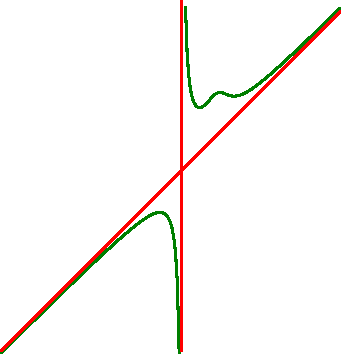
\includegraphics{C2010_1.pdf}
  % C2010_1.pdf: 170x151 px, 72dpi, 6.00x5.33 cm, bb=0 0 170 151
  \caption{Asymptotes}
  \label{fig:C2010_1}
\end{figure}


\subsection{Formule de Stirling}
\index{formule de Stirling} Elle peut être utile dans des problèmes. On la démontrera en exercice. Il est conseillé de la connaitre par coeur.
\begin{displaymath}
  n! \sim \sqrt{2\pi}\, n^n e^{-n} \sqrt{n} .
\end{displaymath}

\end{document}
